\documentclass[../../main.tex]{subfiles}

\begin{document}

\section{Medición de capacitores}

\begin{figure}[H]	
	\centering
	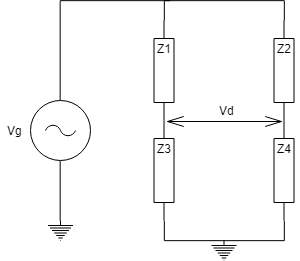
\includegraphics[width=0.35\textwidth]{fotos/PuenteGen.png}
	\caption{Puente con Impedancias genericas} \label{fig:pgc}
\end{figure}

Se diseñó un puente que permita medir capacitores, en un rango de capacidad $C \in [10nF,100nF]$ y en un rango de factor de disipación $D \in[0.015 , 0.09 ] $, para una frecuencia de 10KHz. 
\par Partiendo del puente de la figura \ref{fig:pgc}, donde $V_d=\frac{Z_3}{Z_1+Z_3} -\frac{Z_4}{Z_4 + Z_2}$, en el equilibrio $Z_1 Z_4 = Z_2  Z_3$.  Reemplazando $Z_1= R_1 + \frac{1}{SC_1}$, $Z_2= R_x + \frac{1}{SC_x}$, $Z_3=R_3$ y $Z_4=R_4$. En el equilibrio se cumple que $C_x=\frac{C_1 R_3}{R_4}$, $R_x=\frac{R_1 R_4}{R_3}$ y $D_x=2 \pi f C_1 R_1$.

\subsection{Elección de componentes}
Fijando $C_1=3nF$ y $R_3=1K \Omega$, y a partir de las ecuaciones  $C_x=\frac{C_1 R_3}{R_4}$ y $D_x=2 \pi f C_1 R_1$, se obtuvieron los valores de las variables de ajuste, $R_1 \in \left[  \frac{D_{min}}{2 \pi f C_1 R_1} ,  \frac{D_{max}}{2 \pi f C_1 R_1}  \right] = \left[ 79.5\Omega , 477.46 \Omega   \right]$ y 
$R_4 \in \left[ \frac{C_1 R_3}{C_{Xmax}} , \frac{C_1 R_3}{C_{Xmin}} \right]=   \left[ 30\Omega , 300 \Omega   \right]$.
\par La resitencia $R_1$ se implementó con una resistencia de $68 \Omega$ en serie con dos presets de $200 \Omega$ y la resistencia $R_4$ se implementó con una resistencia de $20\Omega$ en seire con un preset de $200 \Omega$ y otro de $100 \Omega$.

\subsection{Analisis de sensivilidades}

\subsection{Calculo del error}

\subsection{Convergencia}

\subsection{Conclusión}



\end{document}

